\documentclass[a4paper,11pt]{scrreprt}

\usepackage[utf8]{inputenc}
\usepackage[ngerman]{babel}
\usepackage[T1]{fontenc}
\usepackage{amsmath}
\usepackage{graphicx}
\usepackage{xcolor}
\usepackage{wrapfig}
\usepackage{multirow}
\usepackage{ulem}
\usepackage{booktabs}
\usepackage{caption}
\usepackage{subcaption}
\usepackage{url}
\usepackage{fancyhdr}
\usepackage{lscape}
\usepackage{hyperref}
\usepackage{blindtext}
\usepackage{adjustbox}
\usepackage{float}
\usepackage[top=3.5cm,bottom=3.5cm,left=2.5cm,right=2.5cm]{geometry}

\bibliographystyle{unsrt}
\parindent0pt

%Kopf-& Fusszeile----------------------------
\pagestyle{fancy}
\lhead{
\includegraphics[width=1.5cm]{Bilder/fhnw_logo.png}}
\chead{EIT}
\rhead{\slshape \leftmark}
\cfoot{\thepage}
\renewcommand{\headrulewidth}{0.4pt}
\renewcommand{\footrulewidth}{0.4pt}
%--------------------------------------------

\begin{document}
\thispagestyle{empty}

\begin{center}
\begin{tabular}{p{\textwidth}}

\begin{flushleft}

\includegraphics[scale=1.3]{Bilder/FHNW.png}
\end{flushleft}

\\

\\

\begin{center}
\textcolor{black}{
\textbf{
\Huge{
Technisches Pflichtenheft
}}}
\end{center}

\\

\begin{center}
\Large{
\textbf{
Projekt 4
}}
\end{center}

\\

\begin{center}
\large{
Fachhochschule Nordwestschweiz FHNW
}
\end{center}

\\

\begin{center}
\large{\today}
\end{center}

\vspace*{2cm}

\begin{center}
\begin{tabular}{ll}
\toprule 
\textbf{Studiengang:} 		& Elektro- und Informationstechnik EIT \\
\hline
\textbf{Auftraggeber/in:} 	& Prof. Hans Gysin\\
							& Jana Kalbermatter\\
\hline
\textbf{Fachexperten:} 		& Matthias Meier \\
							& Prof. Dr. Pascal Schleuniger \\
							& Pascal Buchschacher \\
							& Dr. Roswitha Dubach \\
							& Dr. Anita Gertiser \\
							& Bonnie Domenghino \\
\hline
\textbf{Projektteam:} & Adrian Annaheim \\ 
							& Benjamin Ebeling \\ 
 							& Jonas Rosenmund\\ 
 							& Michael Schwarz  \\ 
 							& Samuel Wey \\ 
 							& Andres Minder \\ 
\bottomrule
\end{tabular}
\end{center}

\end{tabular}
\end{center}
\newpage

\tableofcontents \thispagestyle{fancy} \cfoot{} \renewcommand{\footrulewidth}{0pt} \rhead{\slshape Inhaltsverzeichnis}
\newpage

\chapter{Auftrag}
% ================ Einstellungen =======================
\thispagestyle{fancy} \setcounter{page}{1} \cfoot{\thepage} \renewcommand{\footrulewidth}{0.4pt} \rhead{\slshape Auftrag}
% ======================================================
Der Besuch eines Kunstmuseums ist weitgehend nicht geführt. Der Besucher bezahlt den Eintritt, ohne zu wissen, was das Museum alles bietet. Für einen Laien resultiert demnach eher ein zielloses Umherschweifen, wodurch sich dessen Fokus weniger auf die bedeutsamen Kunstobjekte richtet. Im Endeffekt bleibt mehr der Besuch in Erinnerung und weniger die Kunstobjekte mit deren Geschichte.
\\[0.5cm]
Der Museumsbesuch kann dem Individuum besser angepasst werden, wie z. B. seinen diskreten Interessen und dessen bevorzugten Sprache. Somit kann nur für die Räume bezahlt werden, welche interessant erscheinen. Anstelle eines gewöhnlichen Tickets soll am Museumseingang ein \textbf{Dojo}\footnote{personalisierbarer Museumsführer} übergeben werden, welches dann die Zutrittsberechtigungen regelt und die Informationen der Kunstobjekte, die sich in der Nähe befinden, über Körperschall\footnote{Übertragung über den Schädelknochen zum Gehör} überträgt. Dadurch wird die Hörbarkeit der Umgebungsgeräusche gewährleistet, anders als bei Kopfhörern. Sollten sich die Ausstellungen des Museums ändern, können einfach neue Daten auf das Dojo geladen werden.
\\[0.5cm]
Bei größerem Interesse des Besuchers an einem Kunstobjekt kann dieser einen \glqq Like-Button\grqq\: drücken und dieses dann quittieren. Beim Zurückgeben des Dojos kann daraus eine persönlich zugeschnittene Museums-History mit den wichtigsten Informationen über die Kunstobjekte zusammengestellt werden.
\\[0.5cm]
Im Verlaufe des Projektes 4 des Studiengangs Elektro- und Informationstechnik geht es um die technische Realisierung des Dojos. Dabei soll das Dojo über einen Akku mit Ladeeinrichtung, Kommunikationsmodule, Bedientasten wie Play/Pause, Lautstärkenregelung und den schon genannten \glqq Like-Button\grqq\: verfügen. Dazu gehören eine Firmware, welche über die Kommunikationsmodule (z. B. Bluetooth) die Zutrittsberechtigungen, wie auch die Ausgabe von Audiofiles (z. B. mp3, wave, ad4) steuert und eine Software, die die allgemeine Verwaltung des Dojos regelt (z. B. Daten Up- bzw. Download von Audiofiles und Likes). 
\newpage

\chapter{Projektziele}
% ================ Einstellungen =======================
\thispagestyle{fancy} \rhead{\slshape Projektziele}
% ======================================================
Als Hauptziel ist die Fertigstellung eines voll funktionfähigen Prototyps gesetzt. Dafür sind die vorerst wichtigsten zu erreichenden Sollziele in der Tabelle \ref{tab:sollziele} aufgezeigt.\\
\section*{Sollziele}
\begin{table}[h]
\centering
	\begin{tabular}{c|c|l}
	\toprule 
	\textbf{Punkt} & \multicolumn{2}{c}{\textbf{Sollziele}} \\
	\hline
	S1 & \multicolumn{2}{l}{Energieversorgung des Dojos mittels Akku} \\
	\hline
	S2 & \multicolumn{2}{l}{das Lokalisieren der Beacons per Bluetooth} \\
	\hline
	S3 & \multicolumn{2}{l}{eine Ladeschaltung des Akkus über USB Typ C} \\
	\hline
	S4 & \multicolumn{2}{l}{Audioausgabe über einen Körperschallaktor} \\
	\hline
	S5 & \multicolumn{2}{l}{die Bedien- und Anzeigeelemente gemäss Design} \\
	\hline
	S6 & \multicolumn{2}{l}{einhalten des Budgets von 200.00 CHF} \\
	\bottomrule 
	\end{tabular}
\caption{}
\label{tab:sollziele}
\end{table}
%%%%%%%%%%%%%%%%%%%%%%%%%%%%%%%%%%%%%%%%%%%%%%%%%%%%%%%%

%%%%%%%%%%%%%%%%%%%%%%%%%%%%%%%%%%%%%%%%%%%%%%%%%%%%%%%%
\section*{Wunschziele}
\begin{table}[h]
\centering
\begin{tabular}{c|c|l}
	\toprule 
	\textbf{Punkt} & \multicolumn{2}{c}{\textbf{Wunschziele}} \\ 
	\hline 
	W1 & \multicolumn{2}{l}{Innenleben des Dojos in den vorgegebenen Massen} \\
	\hline 
	W2 & \multicolumn{2}{l}{Übertragung der Informationen des Like-Buttons auf den PC (Software)} \\
	\hline 
	W3 & \multicolumn{2}{l}{Datendownload und Konfigurationen per Wireless} \\
	\hline 
	W4 & \multicolumn{2}{l}{anbringen einer Kopfhörerbuchse mit 3.5mm für eine sekundäre Audioausgabe} \\ 
	\hline 
	W5 & \multicolumn{2}{l}{Akkulaufzeit mit bis zu mehr als drei Stunden} \\
	\hline 
	W6 & \multicolumn{2}{l}{eine Zutrittskontrolle für bestimmte Räume} \\
	\bottomrule 
	\end{tabular}
\caption{}
\label{tab:wunschziele}
\end{table}	
%%%%%%%%%%%%%%%%%%%%%%%%%%%%%%%%%%%%%%%%%%%%%%%%%%%%%%%%
\newpage

\chapter{Konzept}
% ================ Einstellungen =======================
\thispagestyle{fancy} \rhead{\slshape Konzept}
% ======================================================
\section{Blockschema}
\begin{figure}[h]
\centering
\includegraphics[scale=1.1]{Bilder/p4_flowchart.png}
\caption{Blockschema}
\label{fig:flowchart}
\end{figure}
\vspace*{-0.6cm}
\paragraph*{Aufbereitung:}
Beim Eintritt in das Museum wird das Dojo individuell angepasst. Dafür werden vom PC aus die Audiofiles mit einer dazugehörigen Korrespondenztabelle\footnote{enthält die Zuordnungen der ID. Nummern der BT-Beacons mit den Audiofiles } auf das Dojo geladen. Dabei werden die Audiofiles direkt auf der $\mu$SD-Karte und die Tabelle auf dem internen EEPROM des Mikrocontrollers gespeichert. Wenn der Switch-Block eine Spannung detektiert (Signalpfad vom USB-Switch aus), soll der Datenpfad über die Bridge geschalten sein, damit die $\mu$SD-Karte direkt als Speichermedium auf dem PC angezeigt wird. So kann das Dojo von der PC Software direkt verwaltet und angepasst werden. Ansonsten ist die $\mu$SD-Karte mit dem Audioboard verbunden, damit dieses die Audiofiles abspielen kann.
\newpage
\paragraph*{Benutzung:}
Wenn der Besucher in die Nähe eines Kunstobjektes kommt, soll über das Bluetoothmodul dessen BT-Beacon erfasst werden. In der Firmware des Mikrocontrollers wird über die stärke der Signalleistung des BT-Beacons verifiziert, ob das Objekt nahe genug, oder welches näher ist. Über den Vibrationsmotor und den LEDs wird dann dem Besucher mitgeteilt, dass hier abrufbare Information ist. Gleichermassen wird auch die Zutrittskontrolle erfolgen, indem die empfangenen ID. Nummern der BT-Beacons mit den abgespeicherten abgeglichen werden. Die Objekte können über den Like-Button geliked werden, wodurch die unique ID. Nummer des BT-Beacons im internen EEPROM abgespeichert wird.
\paragraph*{Abgabe:}
Am Schluss können die im int. EEPROM gespeicherten Likes ausgewertet und eine Broschüre mit den Präferenzen des Besuchers zusammengestellt werden.
%%%%%%%%%%%%%%%%%%%%%%%%%%%%%%%%%%%%%%%%%%%%%%%%%%%%%%%%%%%%%%%%%%%%%%%%%%
\section{Hardware}
\subsection{Bluetoothmodul}
Da Beacons in kurzen, regelmässigen Abständen im 2.4 GHz–Band eine Unique ID senden, benötigt das stabförmige Informations-Gerät ein Bluetooth-Modul mit UART-Schnittstelle, um diese Information zu empfangen. Dazu wird ein HC-05 Bluetooth-Modul verwendet. Es ermöglicht das Übertragen der Beacon-Informationen auf den Mikrocontroller, wobei die Bluetooth-Reichweite bis zu 10m beträgt. Der Vorteil eines vorgefertigten Moduls liegt in der einfachen Ansteuerung Hardware-, sowie Firmwareseitig.

\subsection{BT-Beacon}
Der Beacon ist die Bluetooth-Technologie von morgen. Diese kleinen Geräte können an den Ausstellungsstücken als Signalgeber im Museum angebracht werden. Für dieses Projekt wird ein Minew E7 Bluetooth Beacon verwendet, da dieser Beacon über die zwei bekanntesten Protokolle iBeacon und Eddystone verfügt. In der zugehörigen kostenlosen Konfigurations-App kann eingestellt werden, welches Protokoll gesendet wird. Der Beacon kann auch beide Protokolle gleichzeitig senden, bei Bedarf mit unterschiedlichen Signalstärken und Sendeintervallen. Ausserdem hat dieser Beacon eine Reichweite von 100m, ist wasserfest und verfügt sogar über einen Temperatursensor.
\subsection{ICSP-Header}
\begin{wrapfigure}{r}{0.3\textwidth}
	\vspace{-40pt}
  	\begin{center}
		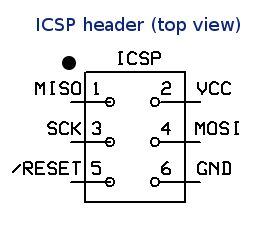
\includegraphics[scale=0.6]{Bilder/icsp_header.png}
  	\end{center}
 	\vspace{-20pt}	
	\caption{ICSP-Header}
  	\vspace{-10pt}
	\label{fig:icsp_header_topview}
\end{wrapfigure}
Damit die Firmware auf dem Dojo bearbeitbar bleibt, wird ein ICSP\footnote{In-Circuit-Serial-Programming}-Header verwendet (oder auch ISP\footnote{In-System-Programming}) \cite{ispwiki}. Damit besteht die Möglichkeit, den Mikrocontroller nach der Installation in das komplette System des Dojos programmierbar zu halten. Über eine SPI-Kommunikationsschnittstelle wird der ICSP-Header an den Mikrocontroller angeschlossen. In der Abbildung \ref{fig:icsp_header_topview} sind die Pinanschlüsse eines sechspoligen ICSP-Headers zu sehen.
\newpage
\subsection{Audioboard}
Das Audioboard beinhaltet den WTV020SD-20S Audiochip. Dieser ist ein kleiner und einfacher IC für die Wiedergabe von Audiofiles. Nach Datenblatt sind mehrere unterschiedliche \textit{Modes} möglich, wobei für das Dojo der \textbf{two line serial mode} verwendet wird. Somit kann der WTV020SD Chip über den Mikrocontroller gesteuert werden und dann Audiofiles, egal welcher Adresse auf der $\mu$SD-Karte abspielen. Der Audiochip ist kompatibel für $\mu$SD-Karten mit Speicherkapazitäten bis zu 1GB. 
\subsection{Audiooutput}
Hierfür wird ein Knochenleiter (Bone conductor) verwendet. Dieser übermittelt das Audiosignal über Körperschall des Schädelknochens an das Gehör weiter.
\subsubsection{Knochenleiter}
Der Knochenleiter\footnote{den von den Dozenten zur verfügung gestellten Knochenleiter} wurde an eine Schaltung mit dem Miniverstärker LM386 angeschlossen, um dessen Verbrauch zu messen. Die Lautstärke wurde als Referenz über einen Laptop geregelt, wobei bei einer Lautstärkeneinstellung von 60 Prozent eine maximale Scheinleistung von 0.263VA und einen Effektivstrom von 0.195A erreicht wurde. Bei dieser Lautstärke ist es für eine klare Audio-Übertragung ausreichend. Für den Energieverbrauch wird mit 0.3W und im worst case Szenario mit 0.5W gerechnet.
\subsection{$\mu$SD-Karte}
Als externes Speichermedium wird eine $\mu$SD-Karte mit einer Speicherkapazität von 1GB verwendet.
\subsection{Tasten}
Für den Nutzer steht auf dem Dojo ein Tastenfeld zur Verfügung:\\
\begin{itemize}
	\item Play/Pause
	\item Volume up/down
	\item Like
	\item Vibro on/off
	\item Power on/off\\
\end{itemize}
\subsection{Energieversorgung}
Das Dojo soll durch einen Li-Ion-Akku mit Energie versorgt werden. Die Akkulaufzeit muss die Dauer mindestens eines Museumrundgangs mit entsprechender Nutzung abdecken, wünschenswert ist eine Akkulaufzeit für einen ganzen Museumstag. Ausserdem wird eine USB-Schnittstelle (Typ C) zur Verfügung stehen, um den Akku nach Rückgabe und Auswertung des Dojos wieder aufzuladen. 
\subsubsection{Akku}
Im Handel sind Akkus vom Typ LI14500 mit einem Durchmesser von 14 mm und einer Länge von 50 mm erhältlich. Die Kapazität beträgt meist um 3 Wh, was nach ersten Abschätzungen für die gewünschte Betriebsdauer ausreicht. Die Kriterien für die Auswahl eines Akkus in der Reihenfolge ihrer Gewichtung sind: Kapazität, Zyklenfestigkeit, Schnellladefähigkeit (nur falls die Kapazität nicht für einen gesamten Tag ausreicht) und Preis. 
\subsubsection{Ladung}
Die Energie kommt über den USB-Anschluss in das Dojo. Da der Strom beim USB-Anschluss standardmässig auf 100 mA begrenzt ist, wird das Dojo mit der entsprechenden Kommunikations-Einheit ausgerüstet, um potentiell leistungsfähigeren USB-Stromquellen bis zu 1.5 A zu entlocken. Die Ladung kann über jeden beliebigen USB-C-Anschluss erfolgen. Um die Ladeinfrastruktur im Museum aufgeräumt und übersichtlich zu halten, ist eine Dockingstation vorgesehen, welche bis zu 50 Dojos aufnehmen kann. 
\section{Software}
\subsection{Software Mikrocontroller}
Die Software soll möglichst schlank gehalten werden.
Zu diesem Zweck benützt der Prototyp den Mikrocontroller eines Arduino UNO's und ein HC-05 BT-Modul.
Der Mikrocontroller steuert das Audioboard, das BT-Modul, die Status LEDs und den Vibrationsmotor.\\[0.5cm]
Der Prototyp benutzt ein Arduino UNO-Board, für das fertige Produkt wird der Mikrocontroller des Arduino UNO's auf einen custom Print gesteckt.
\\[0.5cm]
Für jeden Besucher wird über eine serielle Schnittstelle ein Profil geladen, das beschreibt, welche Audiodatei zu welchem Bluetoothbeacon gehört. \\
Während dem Besuch steuert der Mikrocontroller, welche Datei abgespielt werden soll, je nach dem, bei welchem Beacon der Besucher steht.\\
Zudem speichert der Mikrocontroller, welche Beacons geliked wurden und nach dem Besuch können die gespeicherten Likes wieder über die serielle Schnittstelle abgerufen werden.\\
\newpage
\subsubsection{Allgemeine Funktionsbeschreibung}
Bluetooth-Funktionen:
\begin{itemize}
	\item getClosestBeacon(): gibt die ID des nächsten Beacons zurück
	\item checkBeacon(id): gibt die Signalstärke des Beacons mit der gefragten ID zurück.
\end{itemize}
\vspace*{0.2cm}
Audioboard-Steuerung:
\begin{itemize}
	\item playTrack(tracknumber): spielt die Audiodatei der Nummer tracknumber ab.
	\item pausePlayback():
	\item resumePlayback():
	\item cancelPlayback():
\end{itemize}
\vspace*{0.2cm}
Interface-Steuerung:
\begin{itemize}
	\item requestManifest():
	\item deliverLikes():
\end{itemize}

\subsection{Software PC}
Über den PC wird das Dojo mit eine seriellen Schnittstelle verwaltet. Er hat alle Audiodateien, in den möglichen Sprachen und für alle Ausstellungen des Museums und stellt für jeden Besucher eine individuelle Korrespondenztabelle zusammen, basierend auf dessen Ticket und Sprachpräferenzen. Diese wird dann über die PC Software auf das Dojo geladen. Am Ende des Besuchs kann die Software die Likes vom Dojo für eine Zusammenstellung (z. B. Broschüre) mit den Interessen des Besuchers downloaden. Die Software wird voraussichtlich in Python programmiert.\\
\newpage

\newpage

\chapter{Testkonzept}
% ================ Einstellungen =======================
\thispagestyle{fancy} \rhead{\slshape Konzept}
% ======================================================
\section{Gesamtsystem}
Der Prototyp wird vom Team getestet, indem ein Museumsbesuch simuliert wird und so jede Funktion gebraucht wird. Es wird überprüft, ob die gewünschten Audiodateien abgespielt werden können. Zudem dürfen die nicht gewählten Dateien nicht abgespielt werden. Die Beacon-Erkennung wird simuliert indem drei Beacons in einem Abstand von ca. einem Meter platziert werden. Durch die Erkennung eines Beacons soll ein Vibrationsalarm ausgelöst werden. Der Beacon welcher dem Empfänger am nächsten ist soll gewählt werden und die dazu hinterlegte Audio Datei muss über den Bone Conductor abgespielt werden. Danach werden allfällige Fehler behoben und der Auftraggeber kann das Gerät testen und entscheiden, ob es den Anforderungen genügt.
\section{Hardware}
Während der ganzen Entwicklungsphase werden die einzelnen Komponenten (Bluetooth, USB/UART, Audioboard, etc.) getestet. Auf dem Print werden sie nacheinander in Betrieb genommen, um zu testen, ob sie auch zusammen funktionieren. Die Akku-Ladeschaltung wird zuerst auf einem Entwicklungsboard aufgebaut und mit einem Widerstand eine Last simuliert. So werden mehrere Lade- und Entladezyklen simuliert bevor die Schaltung im Gerät verbaut wird.
\section{Software}
Mit dem Mikrocontroller werden die sogenannten «Likes» simuliert und an den Computer gesendet. So kann getestet werden, ob die Software die «Likes» empfängt und richtig verarbeitet.
\newpage

\bibliography{Literaturverzeichnis/lit_pflichtenheft}
% ================ Einstellungen =======================
\thispagestyle{fancy} \addcontentsline{toc}{chapter}{Literaturverzeichnis} \rhead{\slshape Literaturverzeichnis}
% ======================================================

\newpage

\chapter*{Anhang}
% ================ Einstellungen =======================
\thispagestyle{fancy} \rhead{\slshape Anhang} \addcontentsline{toc}{chapter}{Anhang}
% ======================================================
\section*{Technische Daten des Dojo-Gehäuse}
\begin{figure}[ht]
    \begin{adjustbox}{addcode={\begin{minipage}{\width}}{\caption{%
    }\end{minipage}},rotate=90,center}
	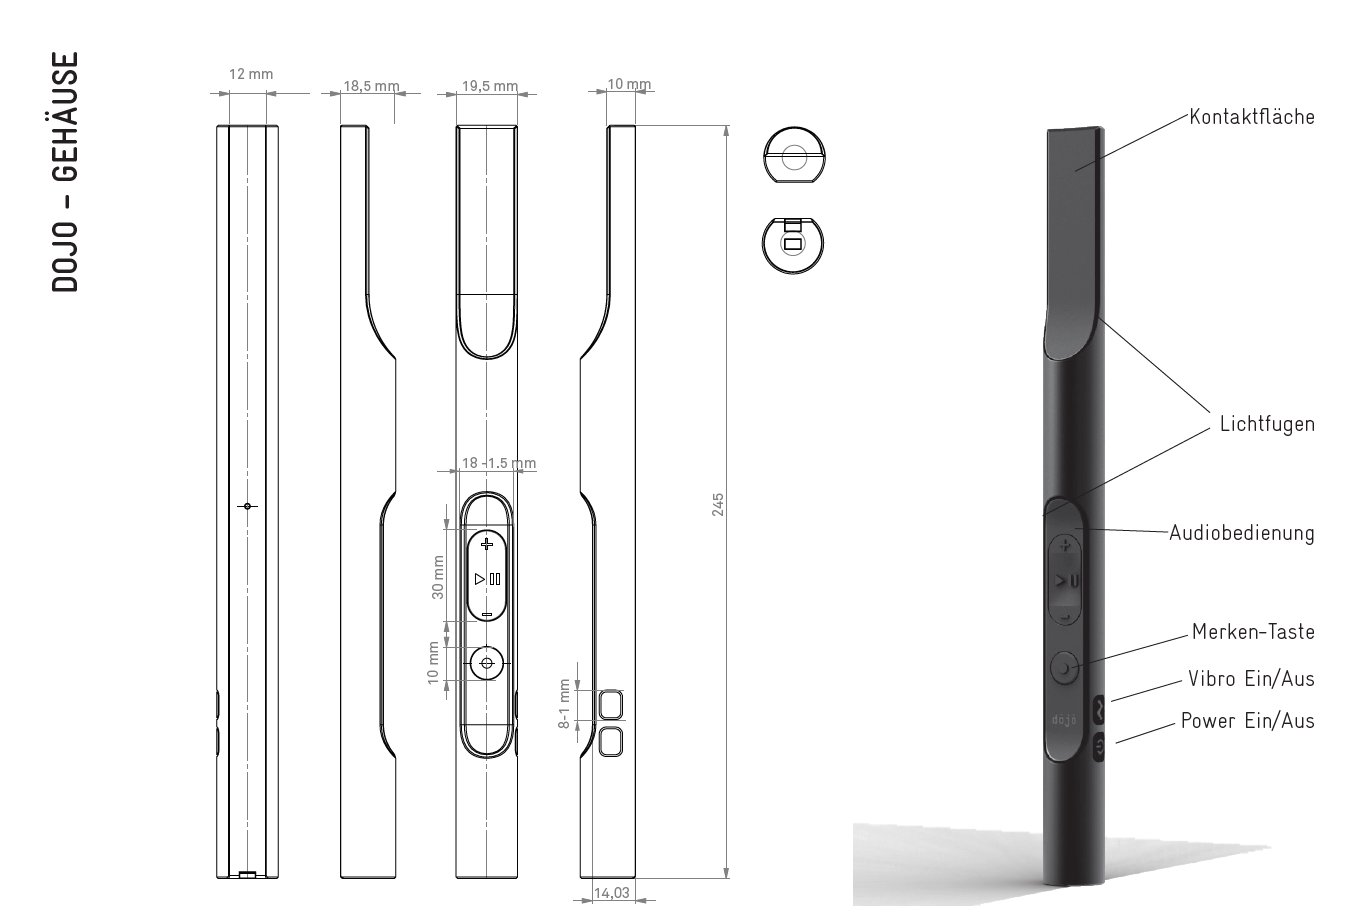
\includegraphics[scale=0.7]{Bilder/dojo_gehaeuse.png} 
	\end{adjustbox}
	\label{fig:dojo_gehaeuse}
\end{figure}
\newpage

\begin{landscape}
\section*{Bauteilliste}
\vspace*{1.5cm}
\begin{figure}[h]
\centering
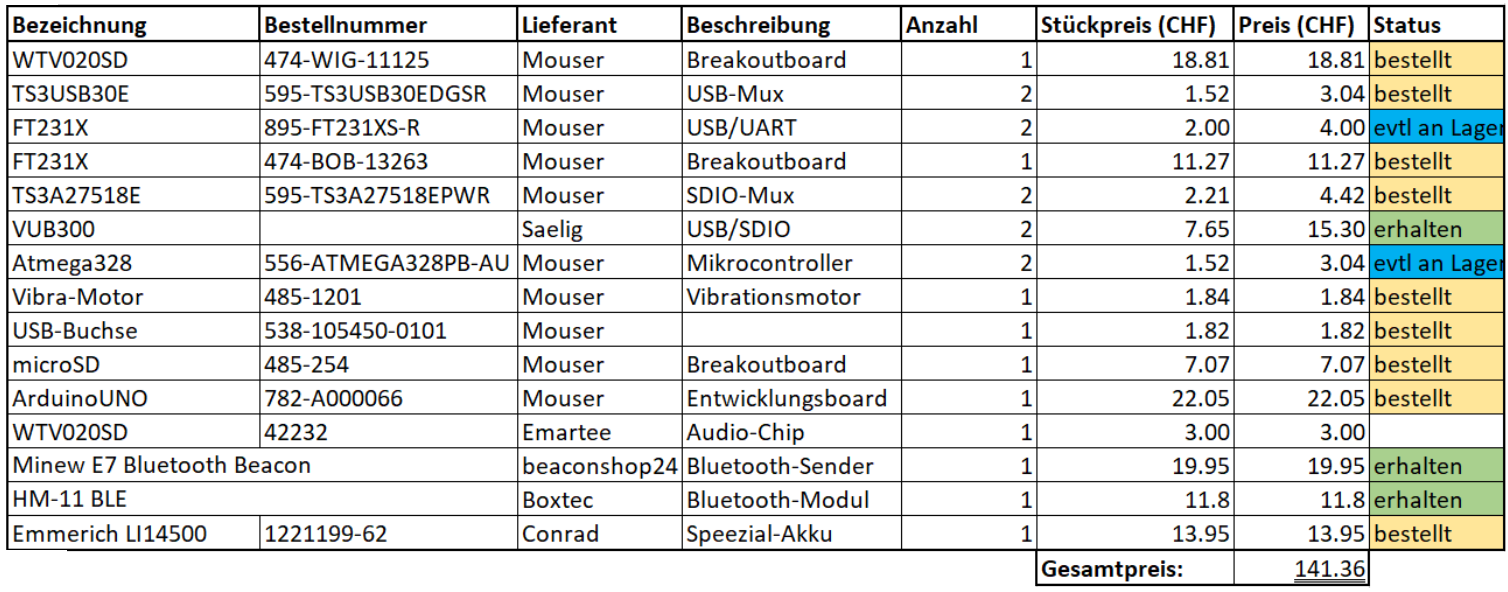
\includegraphics[scale=0.85]{Bilder/bauteilliste.png}
\label{fig:bauteilliste}
\end{figure}
\end{landscape}
\newpage

\end{document}


